% Created 2022-01-21 Fri 12:38
% Intended LaTeX compiler: pdflatex
\documentclass[presentation]{beamer}
\usepackage[utf8]{inputenc}
\usepackage[T1]{fontenc}
\usepackage{graphicx}
\usepackage{grffile}
\usepackage{longtable}
\usepackage{wrapfig}
\usepackage{rotating}
\usepackage[normalem]{ulem}
\usepackage{amsmath}
\usepackage{textcomp}
\usepackage{amssymb}
\usepackage{capt-of}
\usepackage{hyperref}
\mode<beamer>{\usetheme{Madrid}}
\usetheme{default}
\author{M. Falzari}
\date{\today}
\title{Dimensionality Reduction}
\hypersetup{
 pdfauthor={M. Falzari},
 pdftitle={Dimensionality Reduction},
 pdfkeywords={},
 pdfsubject={},
 pdfcreator={Emacs 27.2 (Org mode 9.4.4)}, 
 pdflang={English}}
\begin{document}

\maketitle
\begin{frame}[label={sec:org066413b}]{How?}
\begin{block}<1->{Linear}
\begin{itemize}
\item LDA (Linear discriminant analysis)
\item PCA (Principal component analysis)
\end{itemize}
\end{block}
\begin{block}<2->{Non linear}
\begin{itemize}
\item LLE (Locally linear embedding)
\item Isomap
\item Autoencoder
\end{itemize}
\end{block}
\end{frame}
\begin{frame}[label={sec:org588e26e}]{Why autoencoders?}
\begin{block}{}
\begin{itemize}
\item Autoencoder != other methods
\item Potentially detect repetitive structures
\item \ref{wang2016auto} \ref{lin2020deep}
\end{itemize}
\end{block}
\end{frame}

\begin{frame}[label={sec:org8624603}]{Autoencoder}
\begin{center}
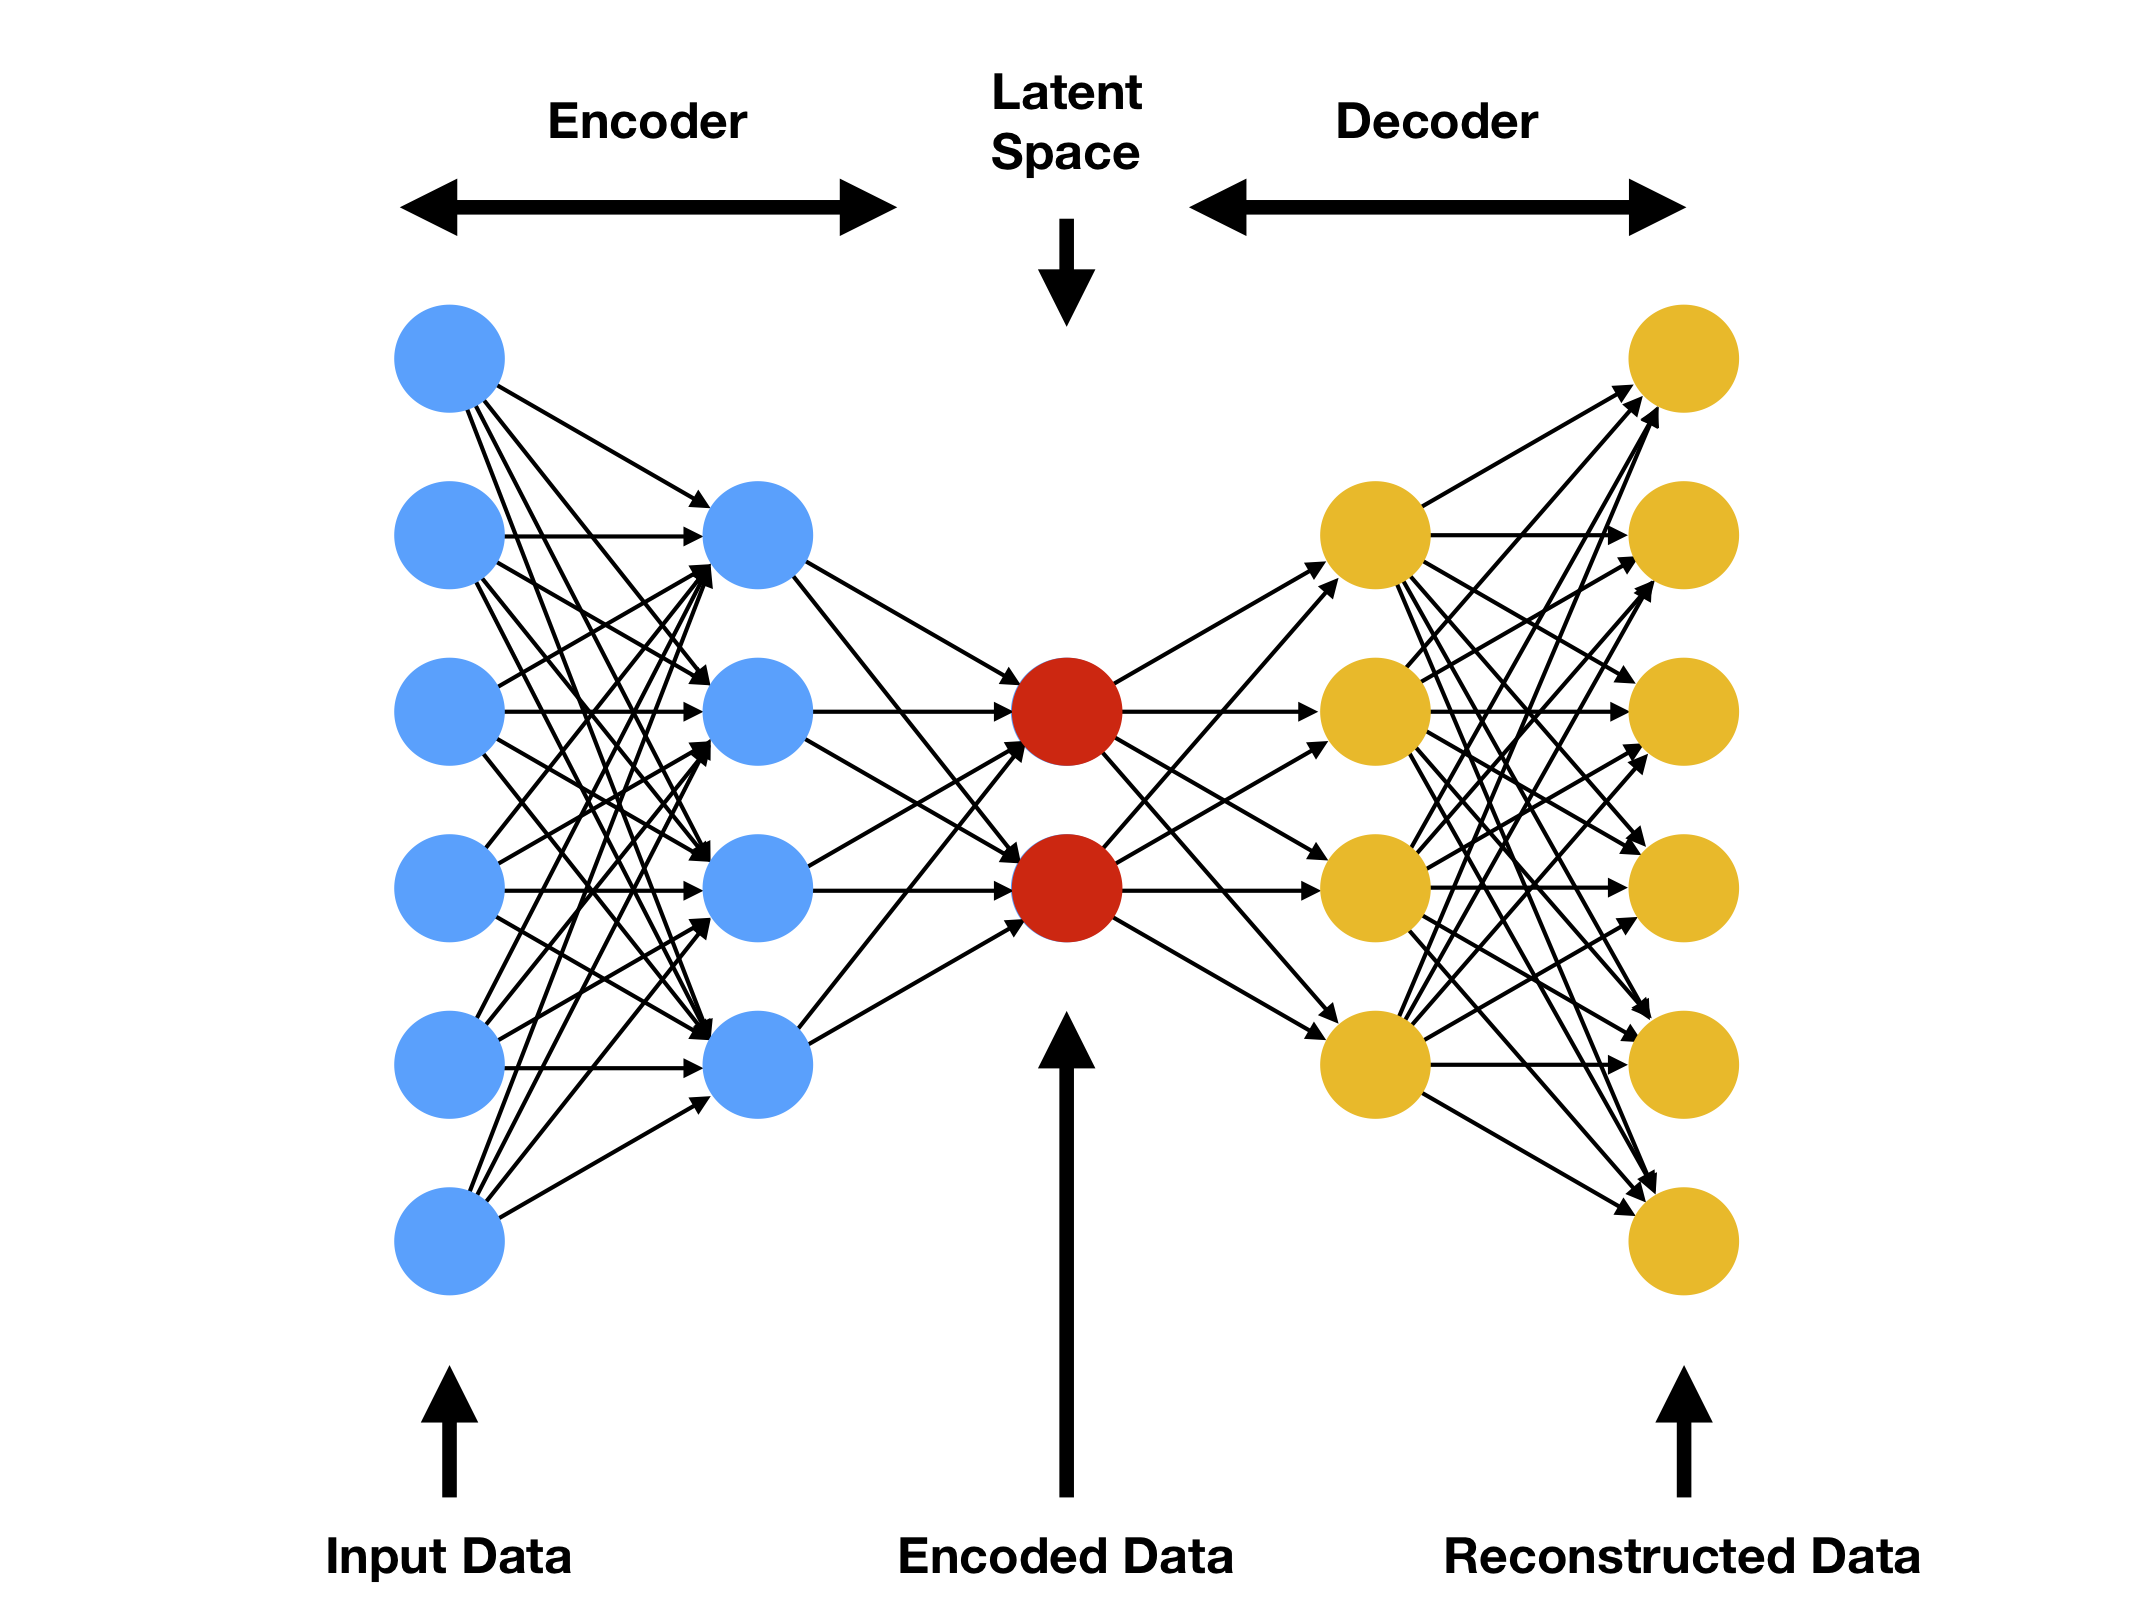
\includegraphics[width=.9\linewidth]{./autoencoder.png}
\end{center}
\end{frame}
\begin{frame}[label={sec:org4d1a420}]{Variational inference}
\begin{block}{Bayesian and Variational inference}
\begin{itemize}
\item find a posterior p(Z|X) such that X = observation and Z latent
variables.
\item (many times) intractable since p(X) is unknown
\item Variational inference try to find a surrogate posterior given a
family of distributions
\item Usually KL(Kullback-Leibler) divergence is used to define how
"close" the surrogate is to the desired posterior.
\end{itemize}
\end{block}
\end{frame}


\begin{frame}[label={sec:org07b2fa5}]{Variational Autoencoder}
\begin{center}
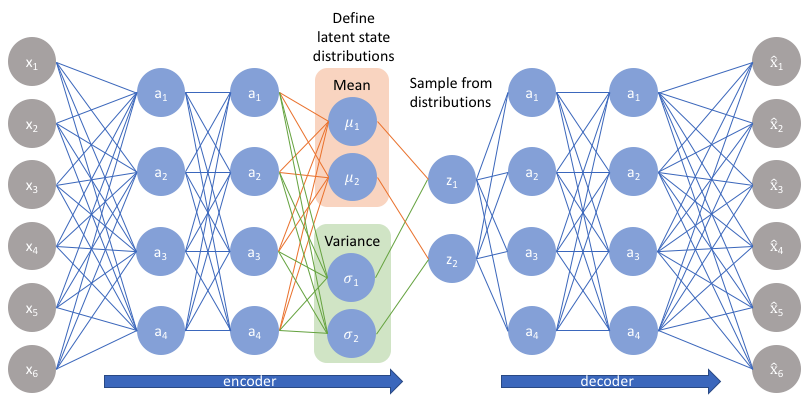
\includegraphics[width=.9\linewidth]{./variational_autoencoder.png}
\end{center}
\end{frame}
\begin{frame}[label={sec:orgce1e7c8}]{Adversarial Variational Bayes}
\begin{block}{}
\begin{itemize}
\item fully implicit latent distribution
\item problematic because KL\textsubscript{div} is intractable
\item use a discriminator in an adversarial manner to approximate the prior
\end{itemize}
\end{block}
\end{frame}

\begin{frame}[label={sec:orge958f05}]{MNIST Example AE}
\begin{center}
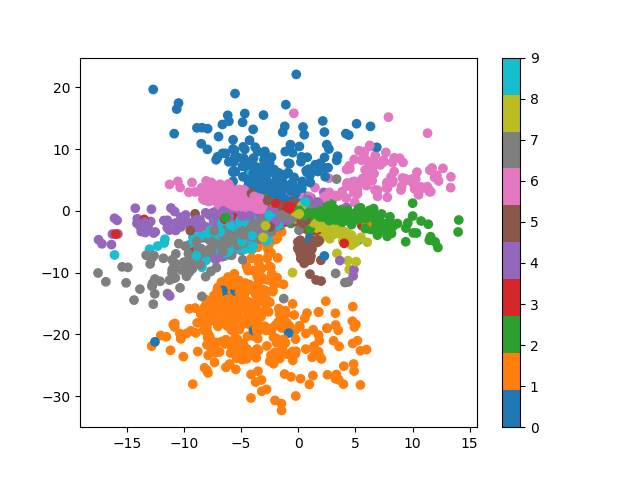
\includegraphics[width=.9\linewidth]{./van.png}
\end{center}
\end{frame}
\begin{frame}[label={sec:orgfa0d697}]{MNIST Example VAE}
\begin{center}
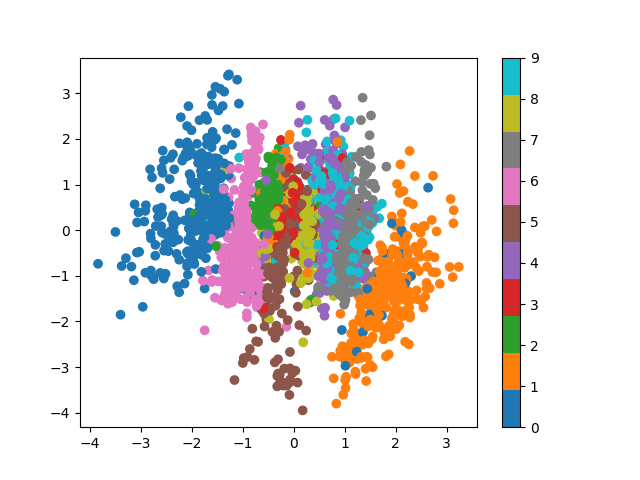
\includegraphics[width=.9\linewidth]{./vae.png}
\end{center}
\end{frame}
\begin{frame}[label={sec:orgc6b61ce}]{MNIST Example AVB}
\begin{center}
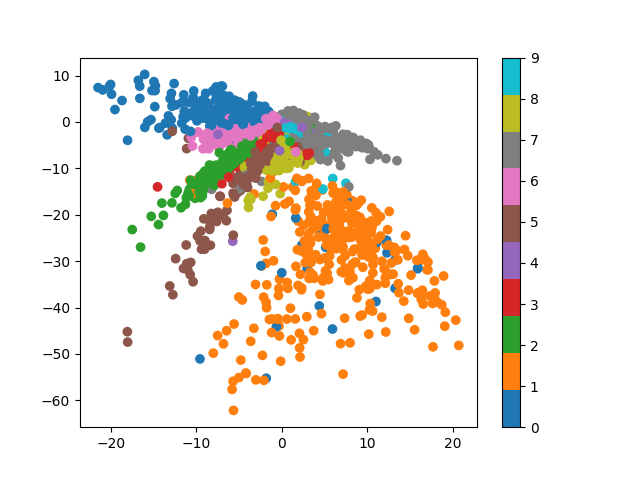
\includegraphics[width=.9\linewidth]{./avb.png}
\end{center}
\end{frame}
\begin{frame}[label={sec:org07a3a5b}]{Training}
\begin{itemize}
\item \ref{higgins2017darla} and others, propose to perform a separate
phase for training the AE "offline"
\item Online
\end{itemize}
\end{frame}

\begin{frame}[label={sec:org889a6af}]{Reference}
\url{./refs.bib}
\end{frame}
\end{document}
